\section{Higher Dimensional Manifolds}

\subsection{Lemmas}
\begin{lem}
\label{lem:manifolds_0}
If \(\DConf_n(\Gamma)\) is an \(m\)-manifold with or without boundary, 
then \(\Gamma\) has at least \(n+m\) vertices and \(n \ge m\).
\end{lem}
\begin{proof}
    If \(\Gamma\) has less than \(n\) vertices, then \(\DConf_n(\Gamma)\) is empty;
    so, suppose \(\Gamma\) has at least \(n\) vertices.
    If \(\Gamma\) has less than \(n + m\) vertices, then
    for any configuration of \(n\) particles on \(\Gamma\)
    at most \(m-1\) particles can simultaneously move.
    Since exactly \(m\) particles need to be able to simultaneously move for an \(m\)-cube 
    to exist in \(\DConf_n(\Gamma)\), no configuration in \(\DConf_n(\Gamma)\)
    can have a neighborhood homeomorphic to an open set in \(\mathbb{R}^m\).

    Similarly, if \(n < m\), then there are not enough particles that can simultaneously move
    for an \(m\)-cube to exist in \(\DConf_n(\Gamma)\). So, \(n \ge m\). 
\end{proof}

Suppose \(\Conf_n(\Gamma)\) is an \(m\)-manifold without boundary and \(n \ge 3\).
By Lemma \ref{lem:manifolds_0}, \(\Gamma\) must have at least \(n + m \ge 2m\) vertices.
Let \(\{v_i w_i\}_{i=1}^{m-1}\) be a collection of \(m-1\) disjoint edges in \(\Gamma\).

\begin{lem}
    \label{lem:manifolds_1}
    For any collection of \(n - m + 1\) vertices \(\{v_i\}_{i=m}^n\)
    in \(\Gamma - \{v_i w_i\}_{i=1}^{m-1}\), there exists exactly two edges
    \(e_1 = v_j u_1\) and \(e_2 = v_k u_2\) such that
    \begin{enumerate}[label=(\roman*)]
    \item \(m \leq j, k \leq n\)
    \item \(u_1, u_2 \not \in \{v_i\}_{i=1}^n\)
    \item Exactly one of the following hold in Figure \ref{fig:lem:manifolds_1}
    \end{enumerate}
\begin{figure}[h!]
    \centering
        \begin{enumerate*}[label=(\arabic*)]
            \item \label{fig:lem:manifolds_1_1}
            \begin{minipage}{.3\textwidth}
                \centering
                \(v_i = v_j\) \textit{and} \(u_1 \neq u_2\) \\
                \vspace{1em}
                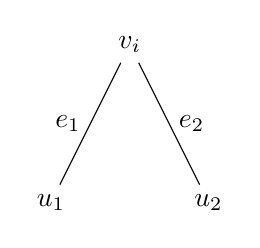
\begin{tikzpicture}
                \node (vi) at (3, 2) {\(v_i\)};
                \node (w2) at (2, 0) {\(u_1\)};
                \node (w3) at (4, 0) {\(u_2\)};
                \draw (vi) -- (w2) node[midway, left] {\(e_1\)};
                \draw (vi) -- (w3) node[midway, right] {\(e_2\)};
                \end{tikzpicture} 
            \end{minipage}
            \hspace{3em}

            \item \label{fig:lem:is_surface_1_1:2}
            \begin{minipage}{.3\textwidth}
                \centering
                \(u_1 = u_2\) \textit{and} \(v_i \neq v_j\) \\
                \vspace{1em}
                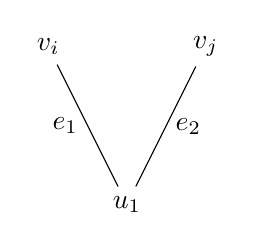
\begin{tikzpicture}
                    \node (vi) at (2, 2) {\(v_i\)};
                    \node (vj) at (4, 2) {\(v_j\)};
                    \node (w2) at (3, 0) {\(u_1\)};

                    \draw (vi) -- (w2) node[midway, left] {\(e_1\)};
                    \draw (vj) -- (w2) node[midway, right] {\(e_2\)};
                \end{tikzpicture}
            \end{minipage}
        \end{enumerate*}
    \caption{Lemma \ref{lem:manifolds_1} possibilities.}
    \label{fig:lem:manifolds_1}
\end{figure}
\end{lem}

\begin{lem}
    \label{lem:manifolds_2}
Let \(\{v_i w_i\}_{i=m}^{n}\) be a collection of \(n-m+1\) vertices in 
\(\Gamma - \{v_i w_i\}_{i=1}^{m-1}\).
The edges \(e_1\) and \(e_2\) guaranteed from applying Lemma \ref{lem:manifolds_1} 
to \(\{v_i\}_{i=m}^{n}\) in the graph \(\Gamma - \{v_i w_i\}_{i=1}^{m-1}\) satisfy exactly one of the following:
\begin{enumerate}[label=(\roman*)]
        \item \(n = m+1\) and these edges belong to a \(Y\)-graph in \(\Gamma - \{v_i, w_i\}_{i=1}^{m-1}\) with two vertices not in \(\{v_i\}_{i=1}^n\).
        \item \(e_1\) and \(e_2\) belong to a \(3\)-cycle in \(\Gamma - \{v_i, w_i\}_{i=1}^{m-1}\) with exactly two vertices not in \(\{v_i\}_{i=1}^n\).
        \item \(e_1\) and \(e_2\) belong to an \(r\)-cycle in \(\Gamma - \{v_i, w_i\}_{i=1}^{m-1}\) with exactly one vertex not in \(\{v_i\}_{i=1}^n\) and \(3 \le r \le (n-m)+2\).
\end{enumerate}

\end{lem}


\begin{lem}
If \(\Gamma - (m-1)K_2\) contains a cycle \(C\), then \(C\) is at most a \(4\)-cycle.
\end{lem}

\begin{lem}
\label{lem:manifolds_C}
If \(\Gamma - \{v_i w_i\}_{i=1}^{m-1}\) contains a cycle \(C\),
then \(C\) is an \((n-m+2)\)-cycle and \(\Gamma - \{v_i w_i\}_{i=1}^{m-1} = C\).
\end{lem}

\begin{proof}
Suppose \(\Gamma - \{v_1, w_1\}\) contains a cycle \(C\).
Suppose that \(C\) has \(r > n-m+2\) vertices and let \(\{v_i\}_{i=m}^n\) be \(n-m+1\) distinct vertices in a path on \(C\).
Let \(u_1\) and \(u_2\) be the vertices adjacent to the endpoints of this path on \(C\) so that
\(u_1\) is adjacent to \(v_m\) and \(u_2\) is adjacent to \(v_n\) but \(u_1, u_2 \not \in \{v_i\}_{i=m}^n\).
Then, the edges \(v_m u_1\) and \(v_n u_2\) contradict the result of 
Lemma \ref{lem:manifolds_1} applied to \(\{v_i\}_{i=m}^n\) in \(\Gamma - \{v_i w_i\}_{i=1}^{m-1}\).
Therefore, \(C\) must have at most \(n-m+2\) vertices.

Suppose instead that \(C\) has \(r < n-m+2\) vertices.  Since \(C\) must have at
least \(3\) vertices to be a cycle, \(3 < n - m + 2\) meaning, \(n > m + 1\).  By
Lemma \ref{lem:manifolds_0}, there must exist at least \(n + m - r\) vertices in
\(\Gamma - \{v_1, w_1\}_{i=1}^{m-1} - C\).  Let \(\{v_i\}_{i=m}^n\) be \(n - m +
1\) vertices in \(\Gamma - \{v_i, w_i\}_{i=1}^{m-1}\) such that the \(r\)
vertices \(\{v_i\}_{i=m}^{m+r}\) are the vertices of \(C\) and the \(n-m-r\)
vertices \(\{v_i\}_{i=m+r+1}^n\) are not on \(C\).

Applying Lemma \ref{lem:manifolds_1} to \(\{v_i\}_{i=m}^n\) in \(\Gamma - \{v_i w_i\}_{i=1}^{m-1}\), 
we obtain two edges \(e_1 = v_i u_1\) and \(e_2 = v_j u_2\).

We claim that neither \(v_i\) nor \(v_j\) can be on \(C\).
To see this, suppose \(v_i\) is on \(C\). 
Now put \(m\) particles on each vertex in \(\{u_1, v_1, \cdots, v_m\}\setminus\{v_i\}\).
As each particle in \(\{v_i\}_{i=1}^{m-1}\) travels to \(\{w_i\}_{i=1}^{m-1}\),
there are three particles that can move to \(v_i\): 
the particle at \(w_2\) and the two particles at the vertices on \(C\) which are adjacent to \(v_i\).
These particles movements result in a book in the configuration space whose
spine corresponds to the movement of the particles at each vertex in \(\{v_i\}_{i=1}^{m-1}\).
Essentially the same argument shows that \(v_j\) cannot lie on \(C\).

Note that \(u_1\) and \(u_2\) cannot be on \(C\) either since 
\(\{v_i\}_{i=m}^{m+r}\) are the vertices of \(C\),
and Lemma \ref{lem:manifolds_1} guarantees \(u_1\) and \(u_2\) do not belong to \(\{v_i\}_{i=1}^m\).

Since \(n > m + 1\), Lemma \ref{lem:manifolds_2} guarantees that \(e_1\) and \(e_2\) belong to a cycle \(D\).

Notice that if \(u_1 \neq u_2\), then putting \(n-1\) particles at each vertex in \(\{v_i\}_{i=m}^n \setminus \{v_m\}\)
and one particle at \(u_2\) allows for \(m+1\) simultaneous movements:
\(m-1\) movements of the particles at each vertex in \(\{v_i\}_{i=1}^{m-1}\),
the movement of the particle on \(C\) adjacent to \(v_m\) to \(v_m\),
and the movement of the particle at \(v_j\) to \(u_1\).
So, \(u_1 = u_2\).

% TODO TODO TODO adjust to m manifold argument....
We claim that there cannot be any edge \(e = u_1 u_2\) such that \(u_1\) is on \(\Gamma - \{v_1, w_1\} - D\) and \(u_2\) is on \(D\).
To see this suppose there did exist such an edge \(e\).
Now put \(n\) particles on \(\Gamma\) so that 
one particle is on \(v_1\), one particle is on \(u_1\), two particles are on \(D - u_2\), 
and \(n - 3\) particles are on \(\Gamma - \{v_1, w_1\} - D - u_1\).
As the particle at \(v_1\) moves to \(w_1\), the particle at \(u_1\) can move to \(u_2\) or 
the one of the two particles on \(D\) at the vertices adjacent to \(u_2\) can move to \(u_2\).
These particles movements result in a book in the configuration space whose spine corresponds to the movement of the particle at \(v_1\) to \(w_1\).

% TODO we can reach a contradiction another way by
% showing that \Gamma - \{v_1, w_1\} = C + D.
% Then, put all n particles on C and D.
% Some movement must be possible so we must then have edges sticking out of the cycles onto v_1 w_1
% But no edge works.
% TODO TODO TODO
Since \(\Gamma\) is connected but \(D\) is not connected to any vertex in \(\Gamma - \{v_1, w_1\} - D\),
there must exist at least one edge connecting an endpoint of \(v_1 w_1\) to \(D\).
Suppose \(e = u_1 u_2\) is such an edge where \(u_1\) is on \(v_1 w_1\) and \(u_2\) is on \(D\).
Put \(n\) particles on \(\Gamma\) so that \(2\) particles are on each endpoint of \(v_1 w_1\), 
\(2\) particles are on \(D - u_2\), 
\(r - 1\) particles are on \(C\), and \(n - r - 3\) particles are on \(\Gamma - \{v_1, w_1\} - D\).
Since \(C\) is an \(r\)-cycle and there are only \(r - 1\) particles on it, 
there exists one particle on \(C\) that can move to another vertex on \(C\).
As this particle moves, the particle at \(u_1\) or one of the two on \(D - u_2\) can move to \(u_2\).
These particles movements again result in a book whose spine corresponds to the movement of the particle on \(C\).
Since surfaces do not contain books, \(C\) must be an \(n\)-cycle.

To see that \(C\) must equal \(\Gamma - \{v_1, w_1\}\) suppose there exists some vertex \(u\) in \(\Gamma - \{v_1, w_1\} - C\).
Since \(C\) is an \(n\)-cycle, \(\Gamma - \{v_1, w_1\}\) has at least \(n + 1\) vertices.
Put particles on \(\Gamma\) so that \(1\) particle is at \(v_1\), \(1\) particle is at \(u\) and \(n-2\) particles are on a path in \(C\).
As seen in the argument for why \(C\) cannot have more than \(n\) vertices, these particles movements correspond to a \(3\)-cube in the configuration
space. Hence \(\Gamma - \{v_1, w_1\}\) must be an \(n\)-cycle.
\end{proof}


\begin{lem}
\label{lem:manifolds_Y}
If \(\Gamma - \{v_i, w_i\}_{i=1}^{m-1}\) does not contain any cycles, then \(\Gamma - \{v_i, w_i\}_{i=1}^{m-1}\) is the \(Y\)-graph.
\end{lem}
\begin{proof}
Suppose that \(\Gamma - \{v_1, w_1\}\) does not contain any cycles.
% TODO
Lemma \ref{lem:is_surface_0} guarantees that \(\Gamma - \{v_1, w_1\}\) contains
at least \(n\) vertices.
Let \(\{v_2, \cdots, v_n\}\) be \(n-1\) vertices in \(\Gamma - \{v_1, w_1\}\)
and apply Lemma \ref{lem:is_surface_1} to \(\{v_2, \cdots, v_n\}\) in \(\Gamma - \{v_1, w_1\}\).
We then obtain two edges we obtain two edges \(e_1 = v_i w_2\) and \(e_2 = v_j w_3\).
Since \(\Gamma - \{v_1, w_1\}\) does not contain a cycle, Lemma \ref{lem:is_surface_2} guarantees that
\(e_1\) and \(e_2\) belong to some \(Y\)-graph \(Y\) and \(n = 3\).

First we show that there can not exist any other vertices in \(\Gamma - \{v_1, w_1\}\) other than those in \(Y\).
Suppose there exists some vertex \(u\) in \(\Gamma - \{v_1, w_1\} - Y\). 
Let \(x\) be the center vertex in \(Y\) that is incident to \(3\) edges.
Now, put 1 particle at \(v_1\), \(1\) particle at \(x\) and \(1\) particle at \(u\).
As the particle at \(v_1\) moves to \(w_1\), the particle at \(x\) can move
to 3 distinct vertices while the particle at \(u\) remains fixed.
These particles' movements result in a book in the configuration space
whose spine corresponds the movement of the particle at \(v_1\) to \(w_1\).
So, every vertex in \(\Gamma - \{v_1, w_1\}\) must belong to \(Y\).

Next we show there cannot be any other edges between vertices in \(\Gamma - \{v_1, w_1\}\)
other than those in \(Y\). Again, let \(x\) be the center vertex in \(Y\).
Since \(x\) is connected to every vertex in \(\Gamma - \{v_1, w_1\}\), if 
there are any additional edges, they must be between vertices other than \(x\).
So, suppose there exists some edge between two vertices \(u_1\) and \(u_2\) in \(\Gamma - \{x, v_1, w_1\}\).
Immediately we reach a contradiction as the vertices in \(\{u_1, x, u_2\}\) now form a \(3\)-cycle.
Therefore, \(\Gamma - \{v_1, w_1\} = Y\).
\end{proof}
